\chapter{Experimental results and discussion}
\label{chap:results}

In this final chapter, we will present and discuss the results obtained through the analysis of various metrics. Initially, we will present the outcomes of all models generated in the conducted experiments (see Section \ref{subsec:experiments}), followed by a more detailed analysis of the top-performing models. 
Furthermore, qualitative representations of predictions will be showcased to enhance the understanding of the models' behavior.



\section{Performances on the test set}
The various configurations of the datasets (see Table \ref{tab:dataset_testing}) have been used to test the models performances.
In this section, with the help of plots, we will analyze the MAE on the test set, dividing it by pollutant, in order to better understand which pollutants' behaviours were better learned  by the models. To evaluate MAE and sMAPE, predictions and the target variables have been rescaled to the original scale.

\subsection{Citypulse}

Of course, as we would expect, results in Citypulse dataset for Ozone and PM\textsubscript{2.5} are almost identical for all models.
Overall (see Figure \ref{fig:aarhus_results}), the most performing models seem to be both LSTMs models, the Dense Encoder Decoder Network, and the Wavelet and TSMixer models. 


\begin{figure}[h]
    \centering
    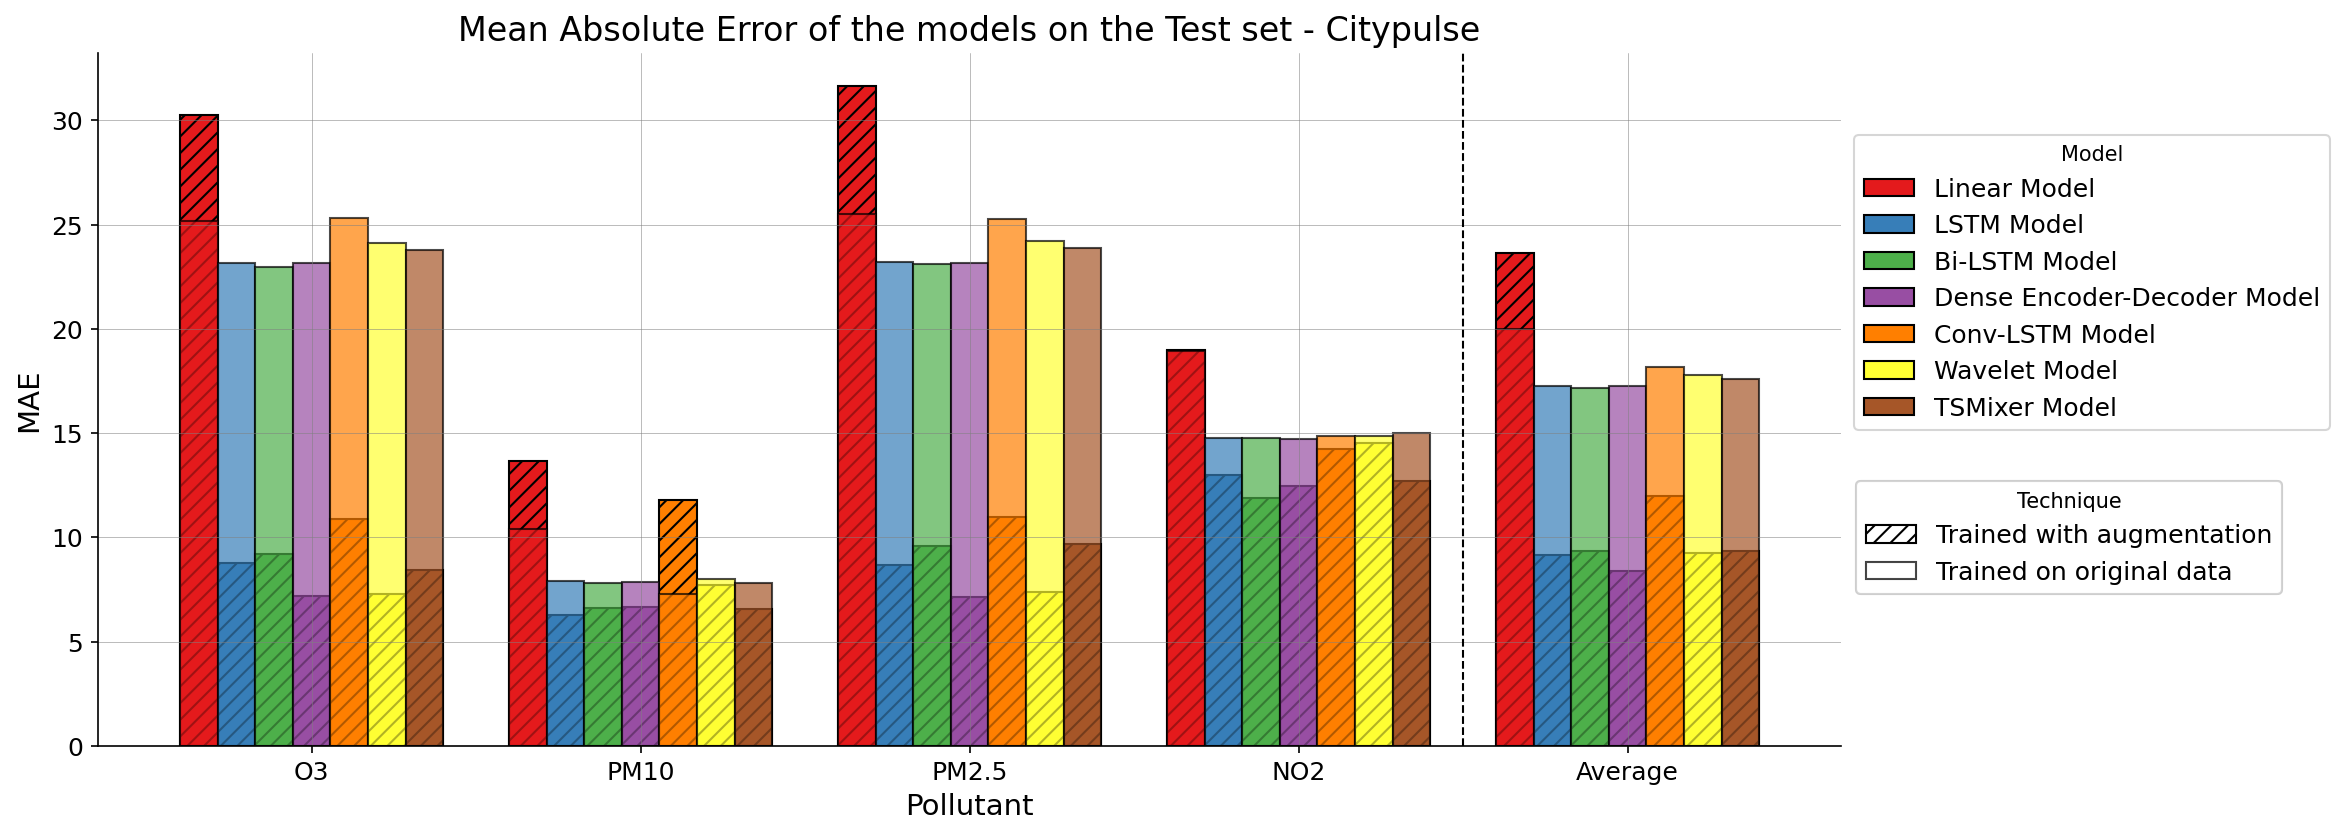
\includegraphics[width=1\linewidth]{images/Aarhus_results.png}
    \caption{MAE on test set, for each model, divided by pollutant. The rightmost graph shows the average MAE of pollutants for each model. Hatched bars represent results after training with augmented data, while solid bars represent MAE without augmented data.}
    \label{fig:aarhus_results}
\end{figure}

It is noteworthy that the linear model does not benefit from the augmentation, exhibiting a higher MAE for all pollutants. This can be attributed to the model's simplicity, as it is unable to adapt to the varying noise injection across epochs and generalize predictions. On average, all models except the linear one yield similar results without augmentation. However, augmentation reveals small differences in the results, but since they are below 1 MAE, it's not enough to select the optimal model for this dataset.
Another aspect that could be noted is that NO\textsubscript{2} and PM\textsubscript{10} presents little differences in MAE in two modalities of training, which could indicate a better predictability of the series.

\begin{table}[h]
    \centering
    \begin{tabular}{lcc}
        \toprule
        \textbf{Model} & \textbf{MAE} & \textbf{sMAPE} \\ 
        \midrule
        Linear & 23,65 & 53.56\% \\
        LSTM & 9,18 & 27.94\% \\
        Bi-LSTM & 9,33 & 27.71\% \\
        \textbf{Dense encoder decoder} & \textbf{8,38} & \textbf{26.38}\% \\
        CONV-LSTM & 11,97 & 34.76\% \\
        TSMixer & 9,34 & 27.81\% \\
        Wavelet & 9,23 & 28.7\% \\ 
        \bottomrule
        \end{tabular}
        \caption{Citypulse models average performances, on augmented dataset models.}
        \label{tab:Citypulse performances}
\end{table}


Ozone and PM\textsubscript{2.5} predictions instead benefits a lot of the augmentation technique. There are two possible explanations for this behaviour:
\begin{enumerate}
    \item The \textbf{collinearity} between the variable is quite reduced by the noise injection, facilitating the models in the prediction task.
    \item Minimizing the loss function could be tricky as each series is independent, and the neural network could focus on minimizing the error for some series, and not improving the others. The noise injection could effectively help the training process in addressing this issue. By introducing controlled random variations or perturbations into the training data through noise injection, the neural network becomes less prone to overfitting on specific series and is better equipped to generalize across diverse sequences.
\end{enumerate}

\subsection{Seoul}

The Seoul dataset yields the best overall results for all models (see Figure \ref{fig:seoul_results}). This is likely due to its consistent observations over time and continuous sensor operation without the need for imputing missing data.

\begin{figure}[h]
    \centering
    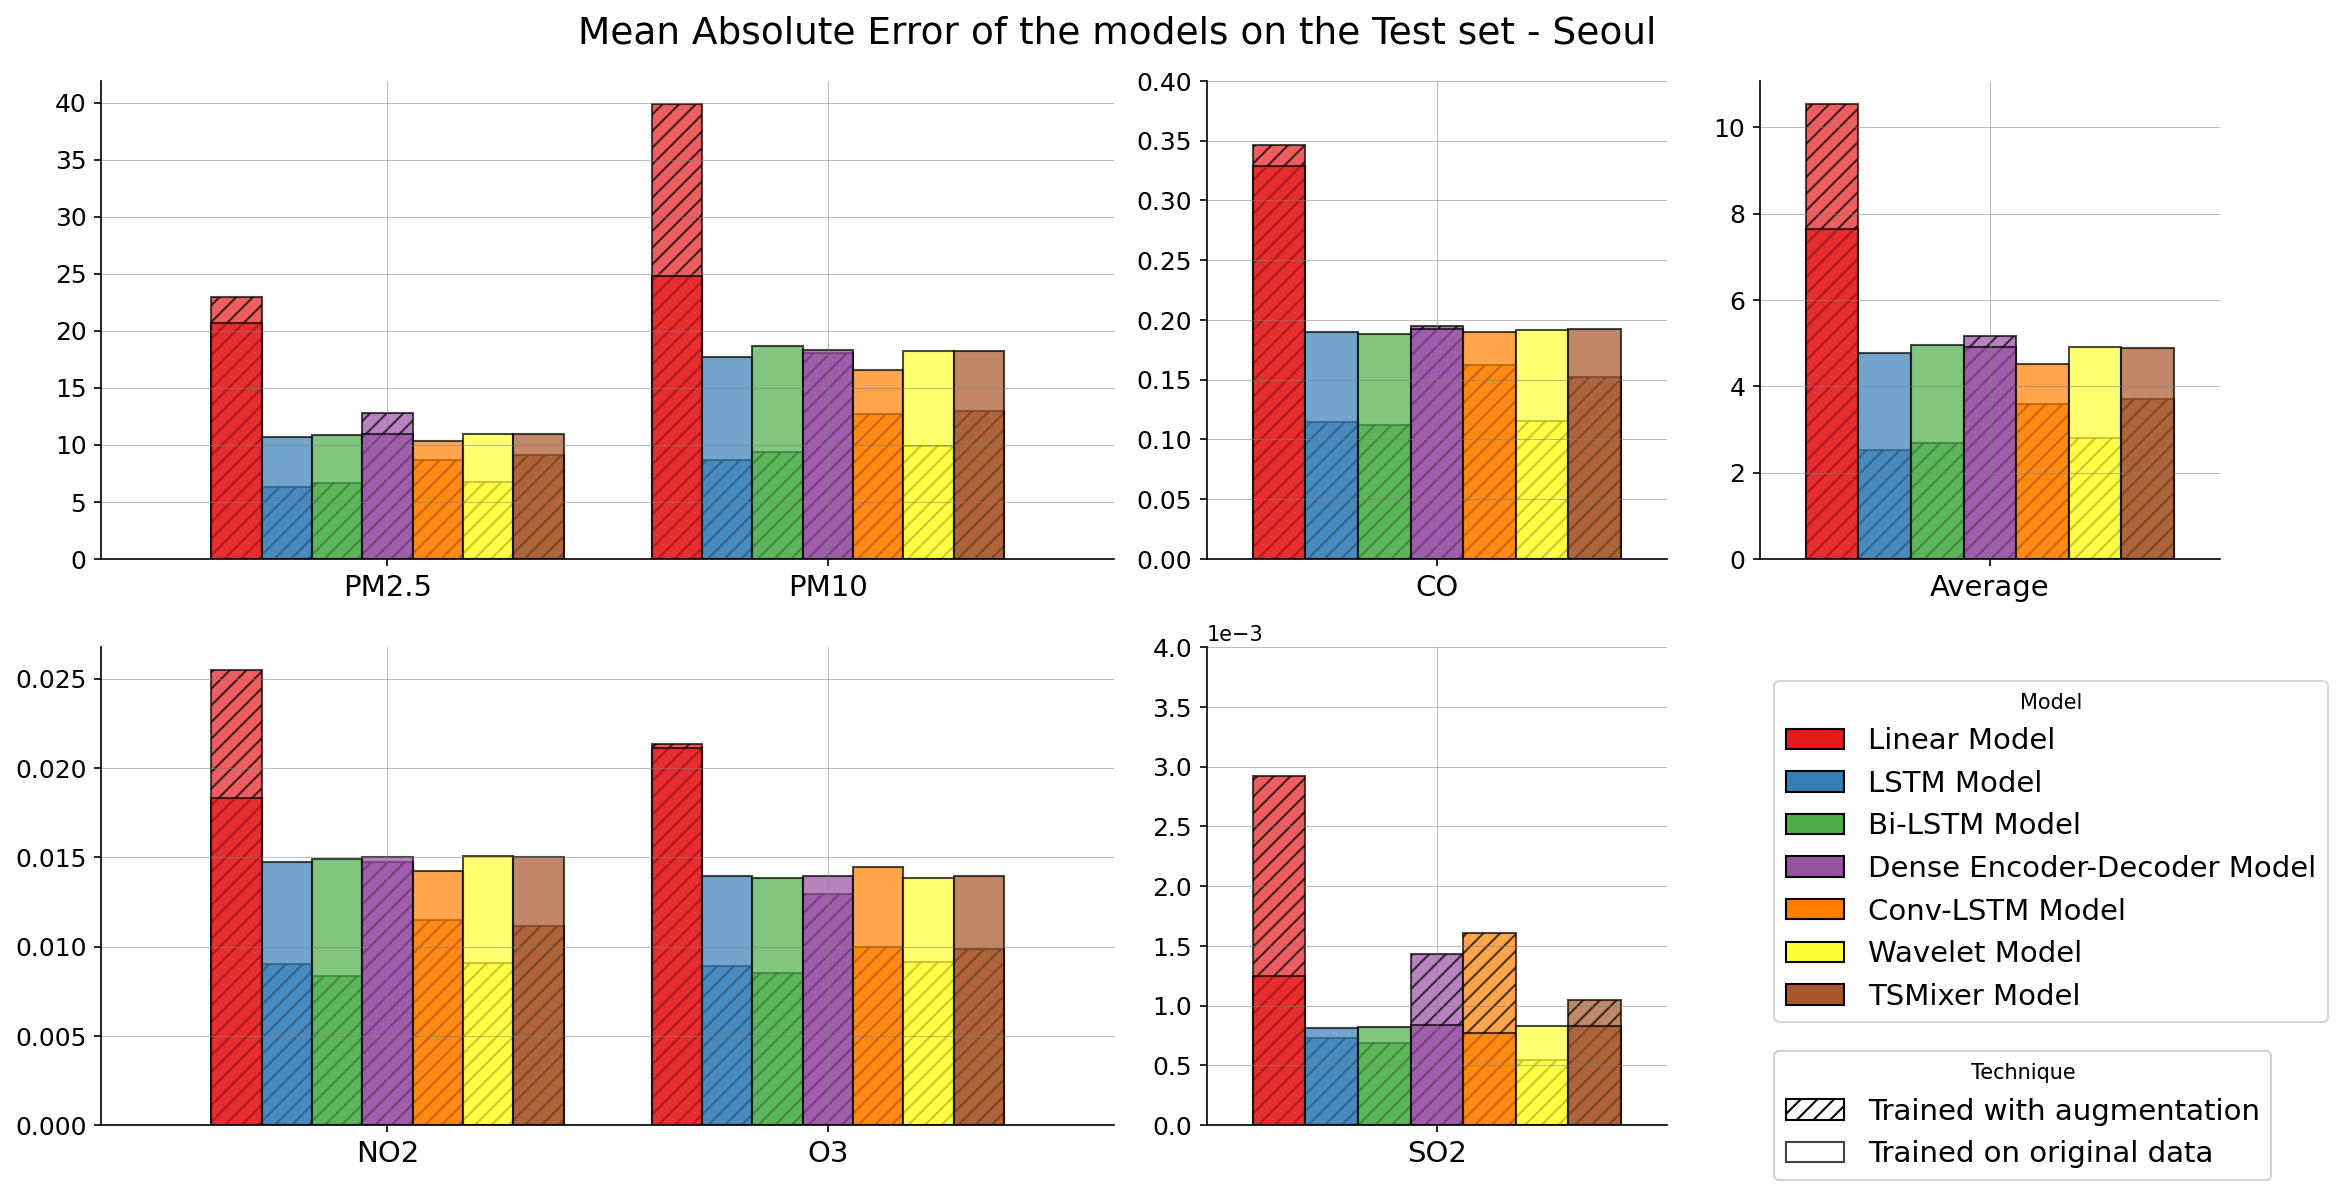
\includegraphics[width=1\linewidth]{images/Seoul_results.png}
    \caption{MAE on test set, for each model, divided by pollutant. The rightmost graph shows the average MAE of pollutants for each model. Hatched bars represent results after training with augmented data, while solid bars represent MAE without augmented data.}
    \label{fig:seoul_results}
\end{figure}

The minimum average MAE encountered is 2.51, in the LSTM model, as we can see in Table \ref{tab:Seoul performances}.
The LSTM, Bi-LSTM, and Wavelet models are the top performers, with a MAE of under 3 and a sMAPE of around 33\%. This is a favorable outcome for real-world applications.

\begin{table}[h]
    \centering
    \begin{tabular}{lcc}
        \toprule
        \textbf{Model} & \textbf{MAE} & \textbf{sMAPE} \\ 
        \midrule
        Linear & 10.55 & 96.93\% \\
        \textbf{LSTM} & \textbf{2.51} & \textbf{33.49}\% \\
        Bi-LSTM & 2.68 & \textbf{33.49}\% \\
        Dense encoder decoder & 5.17 & 51.95\% \\
        CONV-LSTM & 3.60 & 44.18\% \\
        TSMixer & 3.71 & 41.58\% \\
        Wavelet & 2.80 & 33.68\% \\
        \bottomrule
    \end{tabular}
    \caption{Seoul models average performances, on augmented dataset models.}
    \label{tab:Seoul performances}
\end{table}

The linear model exhibits a comparable pattern to the one found in the Citypulse data, which emphasizes its limitations. Despite achieving satisfactory results even in the absence of augmentation, attributed to the substantial volume of training data, the introduction of augmentation enhances performance by an additional 2 points across the top-three models. This reaffirms the potential of augmentation, even in scenarios where ample training data is already available.
Unlike to what is seen in Aarhus dataset, the Dense Encoder-Decoder architecture does not perform as well as the other models. This result suggests weaknesses in learning long and complex patterns.

\subsection{Madrid}

When compared based on sMAPE, the Madrid dataset produced the worst results. Even the previously successful LSTM and Bi-LSTM models now show an sMAPE exceeding 40\%. Additionally, the TSMixer and Wavelet models also exhibit unexpectedly high errors.

\begin{figure}[h]
    \centering
    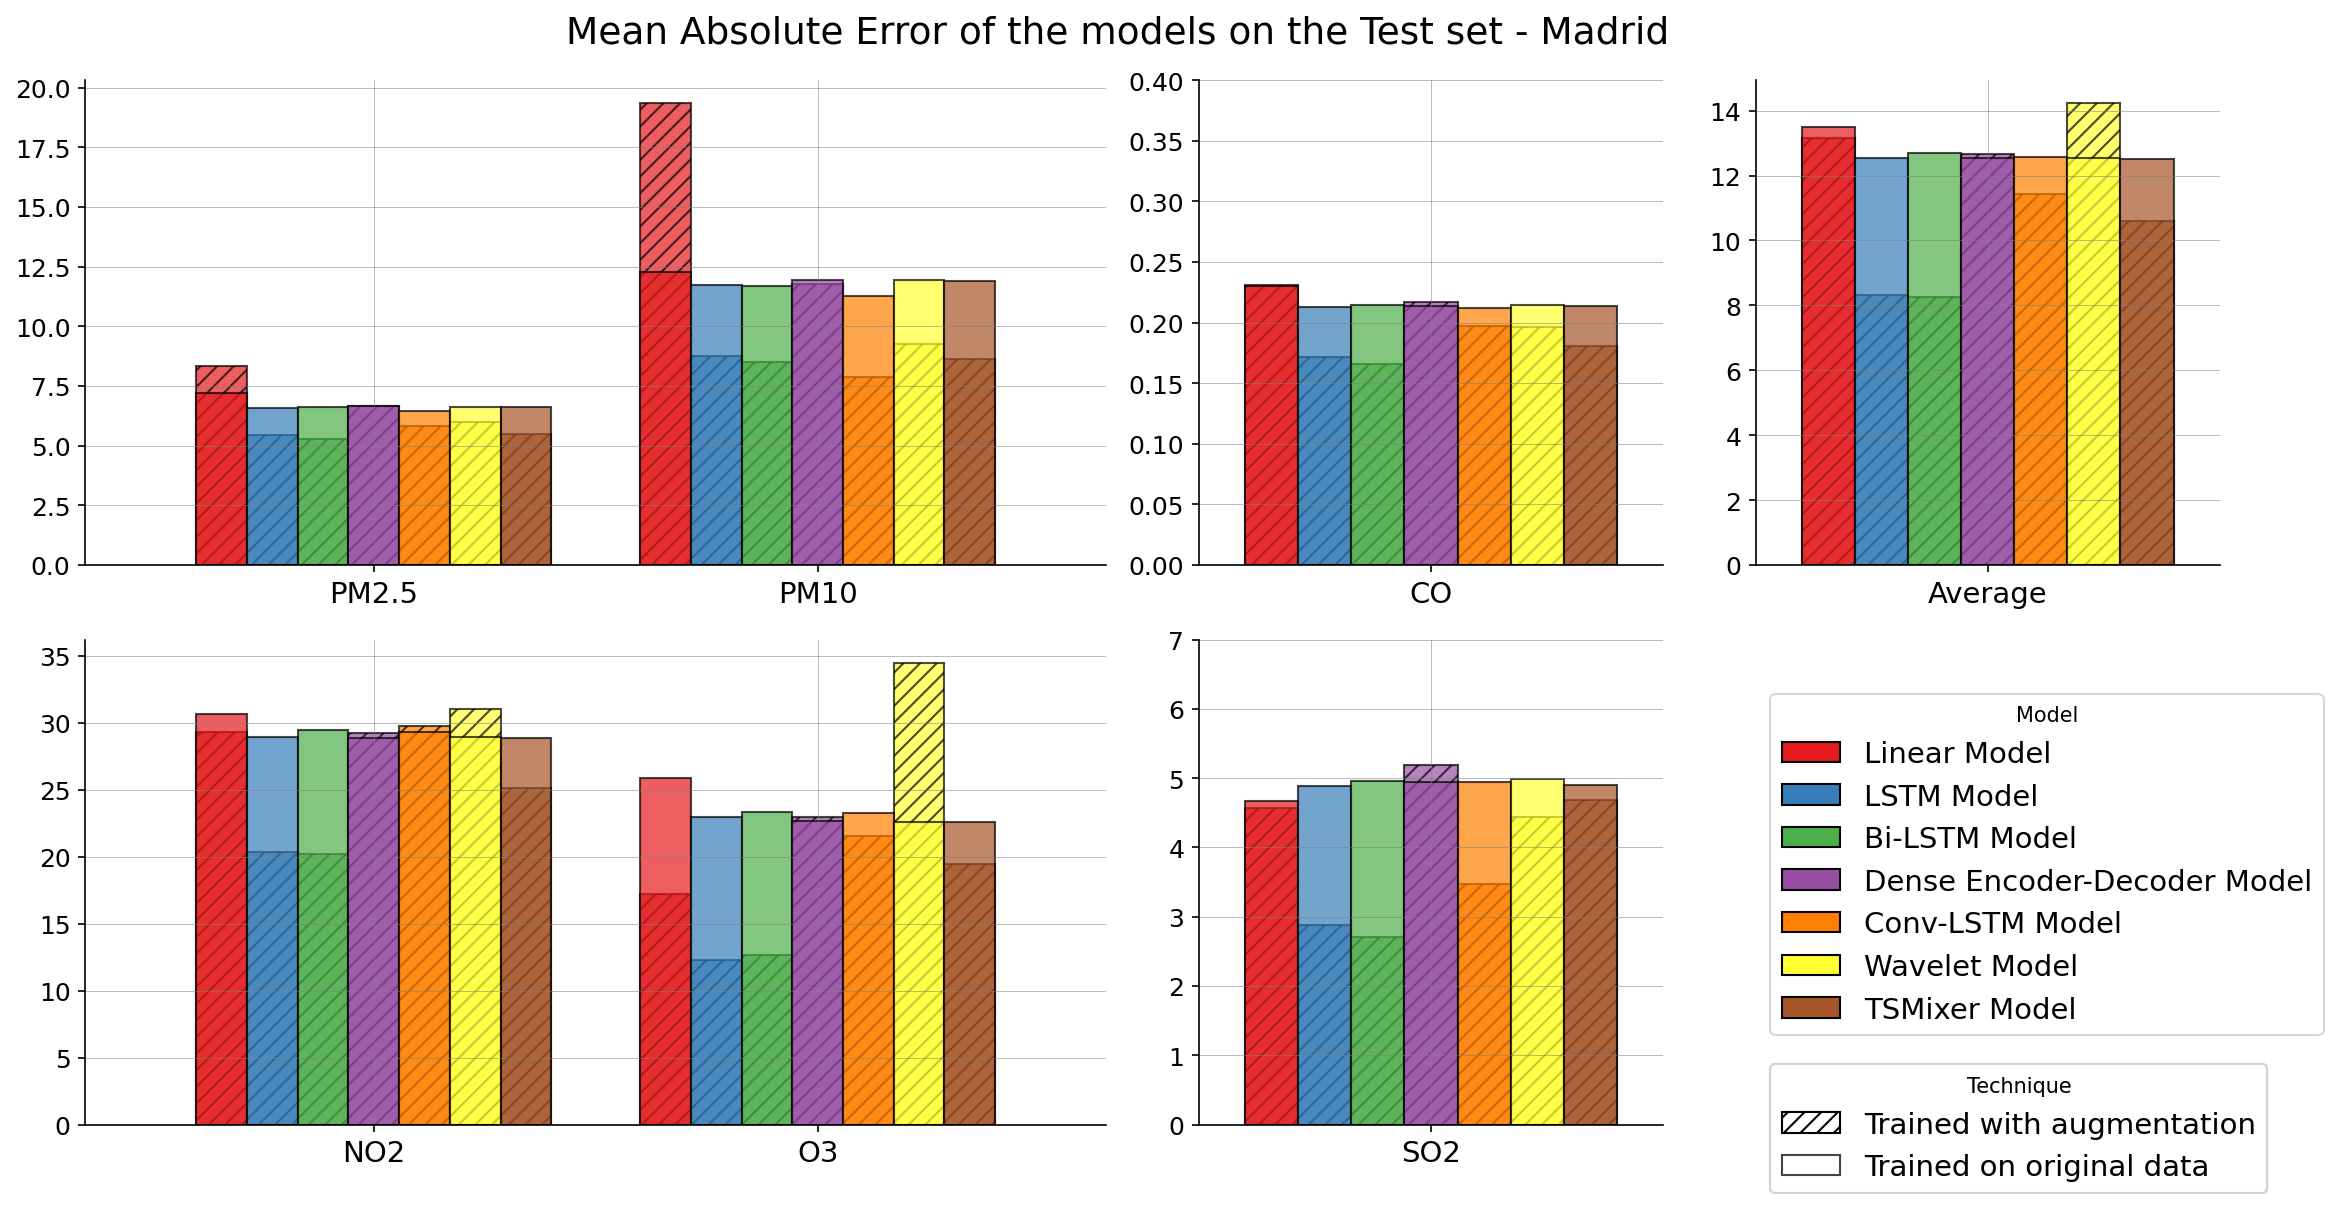
\includegraphics[width=1\linewidth]{images/Madrid_results.png}
    \caption{MAE on test set, for each model, divided by pollutant. The rightmost graph shows the average MAE of pollutants for each model. Hatched bars represent results after training with augmented data, while solid bars represent MAE without augmented data.}
    \label{fig:madrid_results}
\end{figure}

Once again, the Dense Encoder-Decoder model, which previously achieved the best MAE in the Aarhus dataset, is now among the three worst-performing models.
The difficulty encountered can be attributed to the quality of the Madrid dataset, which contains a significant amount of missing data and numerous outliers (as evidenced by the spikes observed in Section \ref{subsec:madrid-eda}). Furthermore, data augmentation does not significantly improve the results, as observed in other datasets, except for the LSTM and Bi-LSTM models, which consistently outperform other models in this experiment.

\begin{table}[]
    \centering
    \begin{tabular}{lcc}
        \toprule
        \textbf{Model} & \textbf{MAE} & \textbf{sMAPE} \\ 
        \midrule
        Linear & 13.17 & 64.3\% \\
        LSTM & 8.31 & 45.03\% \\
       \textbf{Bi-LSTM}& \textbf{8.25} & \textbf{43.95}\% \\
        Dense encoder decoder & 12.66 & 58.49\% \\
        CONV-LSTM & 11.44 & 52.23\% \\
        TSMixer & 10.58 & 51.72\% \\
        Wavelet & 14.23 & 58.02\% \\ 
        \bottomrule
    \end{tabular}
    \caption{Madrid models average performances, on augmented dataset models.}
    \label{tab:Madrid_performances}
\end{table}

The obtained results thus demonstrate a lower predictability of the Madrid dataset, highlighting the necessity for high data quality as well as a substantial amount of data (bearing in mind that in the case of Madrid a 3-year observation period was available).

\section{Best models comparison}

While in the previous section we have showed the performances of all tested models, in this section we will shortly analyze some aspects of the top performing models that should help us to pick the best one for our use case. Choosen top-performing models are the following:
\begin{itemize}
    \item LSTM model
    \item Bi-LSTM model
    \item Tsmixer
    \item Wavelet
\end{itemize}

In this section we will always refer to the results obtained after training with augmentation.

\subsection{Comparison with baseline}
\label{subsec:baseline_comparison}
The Mean Absolute Errors of the highest-performing models were juxtaposed with those obtained from the Autoregressive Integrated Moving Average (ARIMA) models. As elucidated in Section \ref{subsec:baseline}, the baseline's predictions were treated as multiple univariate forecasting problem. To facilitate comparison, the MAE derived from individual series was averaged. It is noteworthy that, in the majority of cases, the baseline tended to predict a linear trajectory, often corresponding to the series mean, rather than exhibiting the expected variability. This predictive behavior of the baseline could indeed contribute to the improvement of MAE.

A summary table (Table \ref{tab:baseline-comparison}) is presented below, delineating the models that surpassed the baseline performance across three datasets.

\begin{table}[]
\centering
\begin{tabular}{lccc}
\toprule
\textbf{Model/Dataset} & \textbf{Citypulse} & \textbf{Seoul} & \textbf{Madrid} \\ 
\midrule
ARIMA & 17.41 & 6.92 & 10.32 \\
LSTM & 9.18 & 2.51 & 8.31 \\
Bi-LSTM & 9.33 & 2.68 & 8.25 \\
TSMixer \cite{chen2023tsmixer} & 9.34 & 3.71 & \textbf{10.58} \\
Wavelet & 9.23 & 2.80 & \textbf{14.23} \\
\bottomrule
\end{tabular}
\caption{MAE table comparison with baseline.}
\label{tab:baseline-comparison}
\end{table}

Evidently, the selected models demonstrate superior performance relative to the baseline in both the Citypulse and Seoul datasets. Conversely, in the Madrid dataset, the TSMixer and Wavelet models fails to surpass the baseline, confirming their inferior performance.

\subsection{Error over time}

The forecast horizon is of course a choice that influences the performances of the models. In the case of one-step-ahead, the model would use the past observations to predict one observation, which would be a quite easy task. During multi-step forecast, the task becomes tricky for two reasons:
\begin{enumerate}
    \item The model has to use the same amount of past observations to predict a longer sequence of observations
    \item The error in one observation can propagate to the successive ones
\end{enumerate}

Of course, the more observations we try to predict, the larger the error.
In the following plot (Figure \ref{fig:mae-per-hour}) we have compared the error of each model, for each dataset, based on the temporal distance from the last observed value.

\begin{figure}
    \centering
    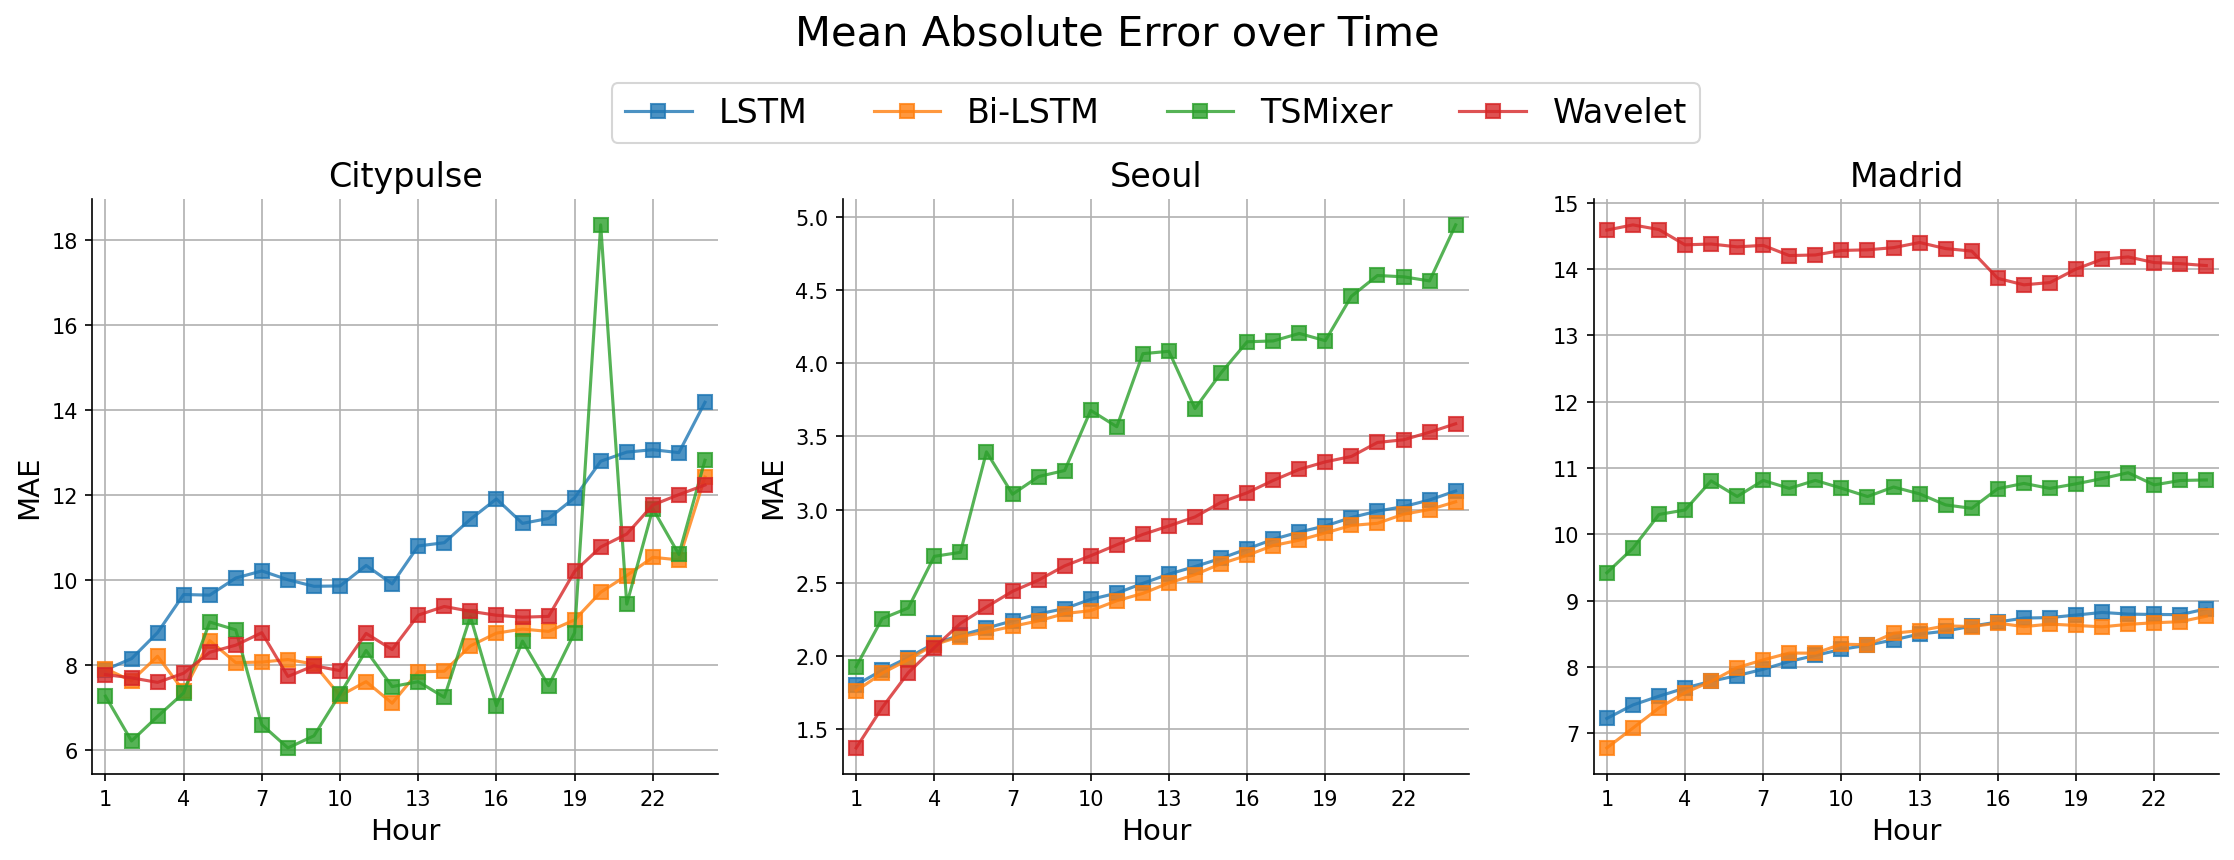
\includegraphics[width=1\linewidth]{images/mae_per_hour.png}
    \caption{MAE of each model based on the distance (in hours) from the last observed value.}
    \label{fig:mae-per-hour}
\end{figure}

Commencing with the Citypulse dataset, a discernible trend is observed, as anticipated, wherein the error exhibits a gradual increase over the forecast horizon. Notably, the Bi-LSTM and TSMixer models emerge as the two most proficient models in managing this aspect. However, while the error in the Bi-LSTM dataset displays a relatively uniform growth pattern, the TSMixer curve manifests substantial variability, casting doubt on the reliability of model predictions.

In the Seoul dataset, results are more transparent and interpretable. While the Wavelet model demonstrates superior predictive capabilities in the initial two observations, it is noteworthy that the error rapidly escalates until approximately the eighth observation. Subsequently, it exhibits a slow and linear growth. In contrast, the curves of the LSTM and Bi-LSTM models, which achieved the best results in terms of both MAE and sMAPE, are nearly overlapping. These models demonstrate a gradual linear worsening, with a minimal increase at the maximum forecast distance. On the other hand, the TSMixer model, despite starting with a relatively low error of approximately 2, deteriorates rapidly towards an error at the maximum distance equal to 5.

In the Madrid dataset, the performance of the LSTM and Bi-LSTM models is reaffirmed, as the error increases gradually with temporal distance. The TSMixer model also achieves an intermediate result, albeit inferior to the baseline (refer to Section \ref{subsec:baseline_comparison}). Conversely, the Wavelet model exhibits a peculiar trend. Despite a slight improvement, the error increases with temporal distance, deviating from the expected decrease. This outcome may be attributed more to chance than to a recognizable pattern.\\

After these considerations, the analysis will focus on the Bi-LSTM and the LSTM models, and we will then analyze the errors and will show some qualitative plots to better understand the behaviours of the two models.

\subsection{Error analysis}

In addition to Mean Absolute Error (MAE), which is a quantitative metric, another valuable approach for assessing errors involves examining the distribution of residuals. A residual is the difference between the predicted and actual values, and by plotting their distribution, insights into the model's performance can be gained. An ideal scenario is one where residuals are concentrated around zero, indicative of accurate predictions. Conversely, a shift in the distribution signals a tendency for the model to either overestimate or underestimate future values.

Figure \ref{fig:kde_residuals} illustrates the residual distributions for both Long Short-Term Memory (LSTM) and Bidirectional LSTM (Bi-LSTM) across the three datasets. Analyzing these distributions provides valuable insights into the models' tendencies to either overestimate or underestimate future values for each dataset.

\begin{figure}
    \centering
    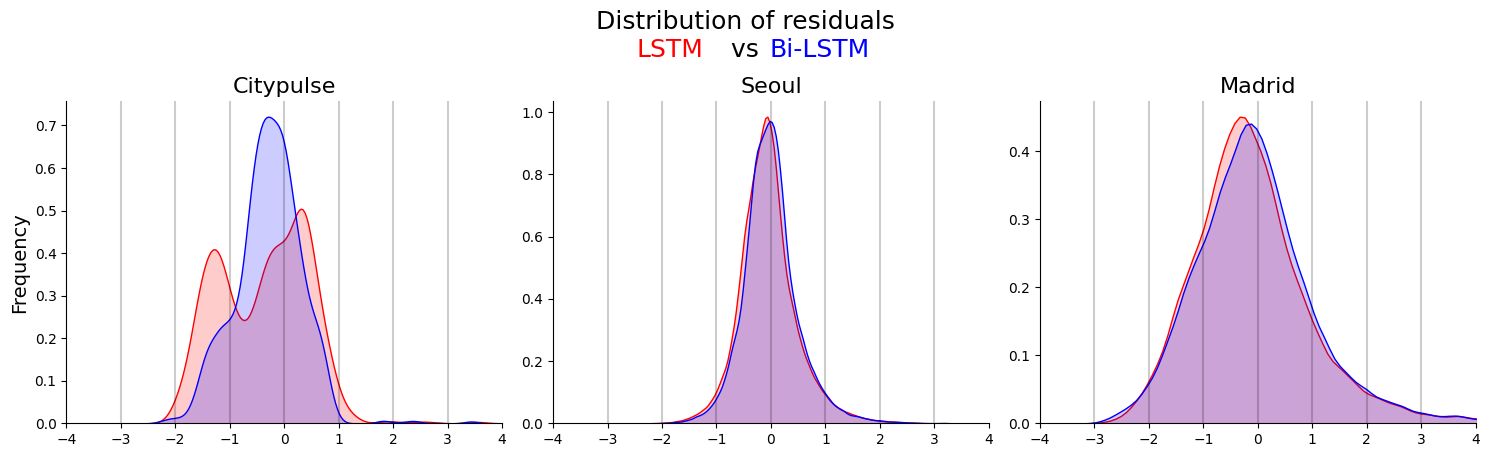
\includegraphics[width=1\linewidth]{images/Residuals_distribution.png}
    \caption{Distribution of residuals for each dataset, LSTM model (in red) and Bi-LSTM model (in blue)}
    \label{fig:kde_residuals}
\end{figure}

The results show differences between the models, especially in the CityPulse dataset. The Madrid and Seoul datasets have similar results for both the Bi-LSTM and LSTM models. In the CityPulse dataset, while the Bi-LSTM model's performance curve is skewed but mostly normal, the LSTM model shows a distribution with two peaks: one near zero and the other at -1.2. This indicates that the model accurately predicts some values while overestimating others.

The complexity of this phenomenon cannot be fully explained by the Mean Absolute Error (MAE), highlighting the need for this analysis. It can be argued that the accuracy of the first peak predictions compensates for the other peak prediction in the MAE calculation, resulting in a close approximation of the Bi-LSTM model's performance.

Next, we will provide concise visual representations of out-of-sample forecasts for both the Bi-LSTM and LSTM models. It is important to note that these plots should not be used as the sole criterion for determining the superior performance of a model. Instead, they should be considered a potential tool for gaining a better understanding of how the information extracted from the previous analysis applies in practice.

\paragraph{Citypulse}
From the plots in Figure \ref{fig:forecasts_aarhus}, we can see that while the Bi-LSTM model (in blue) doesn't fit very well with the predictions, the LSTM model gets better results in O\textsubscript{3} and PM\textsubscript{2.5} series, but overestimates both PM\textsubscript{10} and NO\textsubscript{2} series. If repeated, this pattern could explain the difference seen in the distribution of residuals.

\begin{figure}[h]
    \centering
    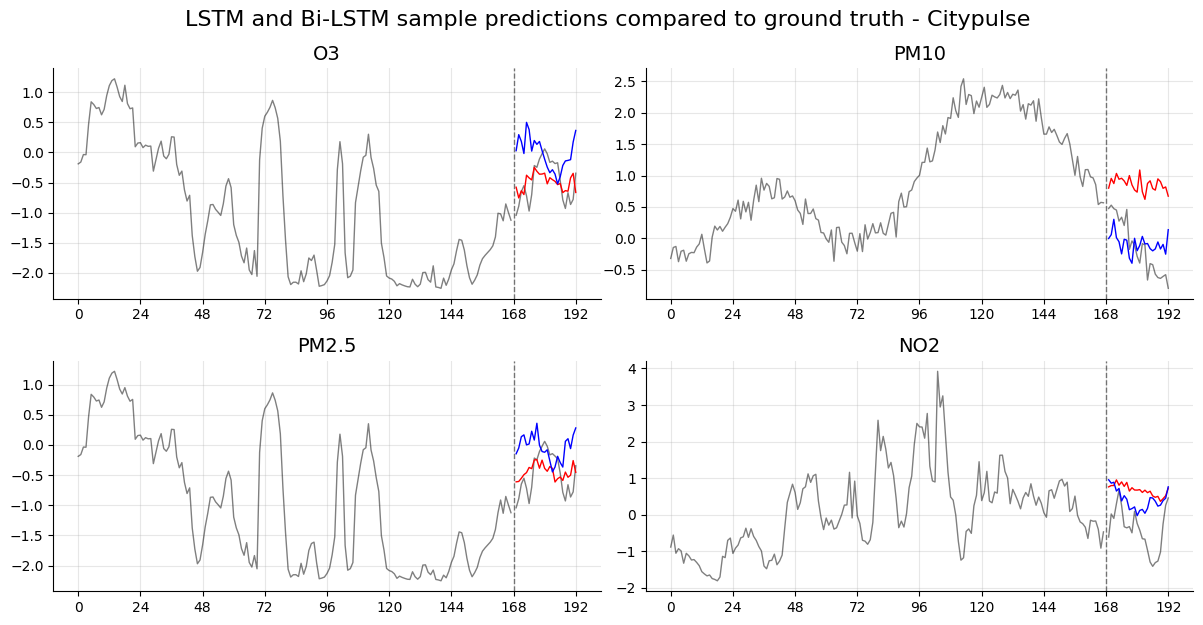
\includegraphics[width=1\linewidth]{images/forecasts_aarhus.png}
    \caption{Forecast of one time window extracted from the test set of Seoul dataset. Both models forecasts are displayed, LSTM (in red) and Bi-LSTM (in blue)}
    \label{fig:forecasts_aarhus}
\end{figure}

\paragraph{Seoul}

The predictions delineated in Figure \ref{fig:forecasts_seoul} elucidate a marked parity between the two models, evident in their capacity to encapsulate the overarching trend within the series. It is noteworthy that this congruence extends to both O\textsubscript{3} and CO predictions, wherein the forecasted trajectories closely mirror those of the original series.

\begin{figure}[h]
    \centering
    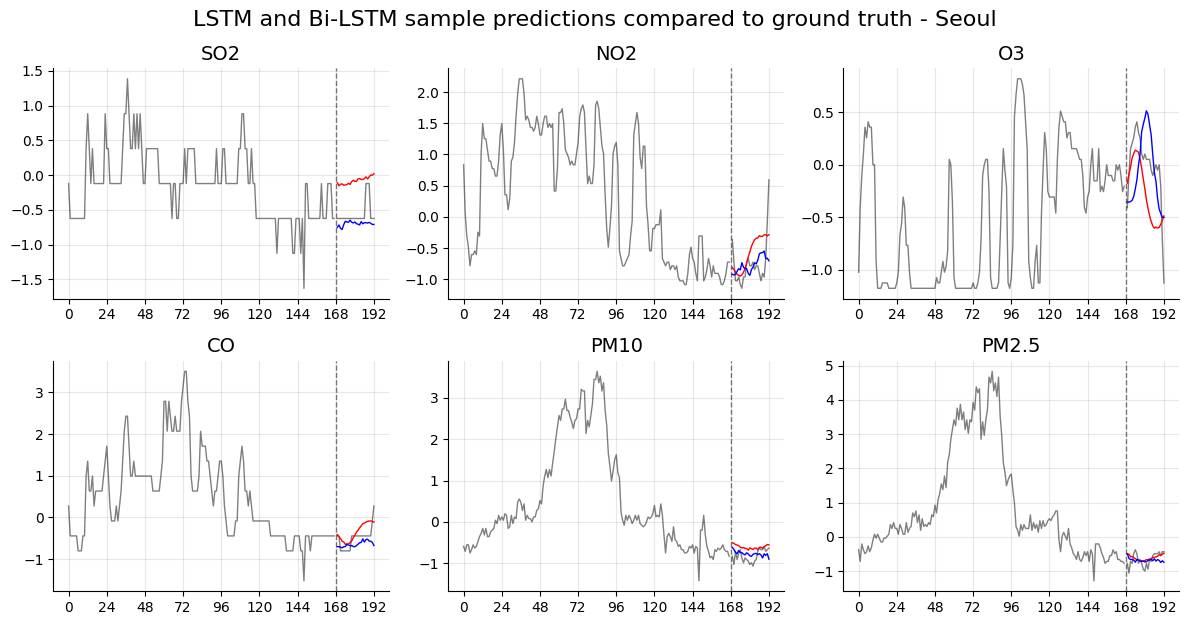
\includegraphics[width=1\linewidth]{images/forecasts_seoul.png}
    \caption{Forecast of one time window extracted from the test set of Seoul dataset. Both models forecasts are displayed, LSTM (in red) and Bi-LSTM (in blue)}
    \label{fig:forecasts_seoul}
\end{figure}

\paragraph{Madrid}
The dataset from Madrid exhibits the most variability, as shown in the plots in Figure \ref{fig:forecasts_Madrid}. However, the models provide a reasonably accurate approximation of future values, particularly the Bi-LSTM model. The SO\textsubscript{2} series has the poorest predicted values, as the models fail to accurately predict actual values. It is worth noting that the SO\textsubscript{2} series appears to have a step function shape, unlike the other series.

\begin{figure}[h]
    \centering
    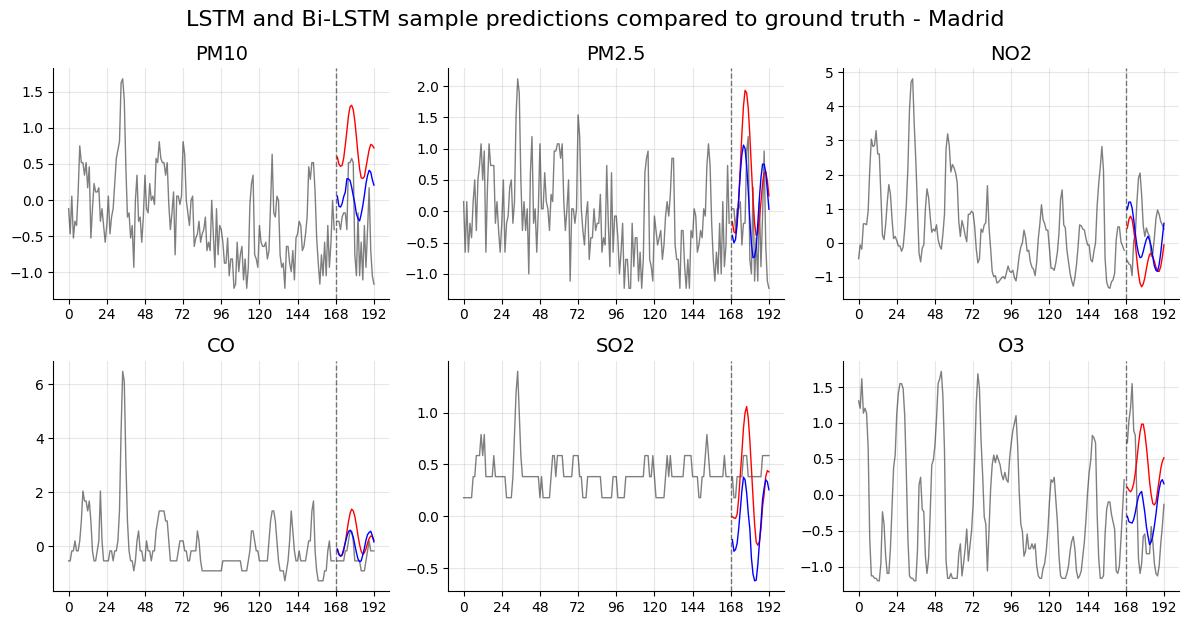
\includegraphics[width=1\linewidth]{images/forecasts_madrid.png}
    \caption{Forecast of one time window extracted from the test set of Madrid dataset. Both models forecasts are displayed, LSTM (in red) and Bi-LSTM (in blue)}
    \label{fig:forecasts_Madrid}
\end{figure}

\section{Results discussion}

In this research, seven models were tested on the three existing datasets. These experiments provided a more comprehensive understanding of the requirements for proficient time series prediction using deep learning models which are often referred to as black-boxes\footnote{This term is used to describe their lack of transparency in the decision-making process}.

\subsection*{Ablation studies}

The study shows that models that take into account temporal considerations, such as memory mechanisms (as seen in LSTM, Bi-LSTM, and Wavelet models) or features derived from the temporal dimension (as seen in TSMixer), consistently outperform other models in terms of predictive efficacy.

Various configurations of the data fed into the training phase have been tested:

\paragraph{Historical data volume influence}

As described in Section \ref{subsec:experiments}, we investigated the impact of historical data volume on the models trained on Seoul and Madrid datasets. Specifically, we compared the outcomes of models trained on a 1-year temporal span with those trained over a 3-year interval without augmentation. The results are presented in Figure \ref{fig:more_data_improv}.

\begin{figure}[h]
    \centering
    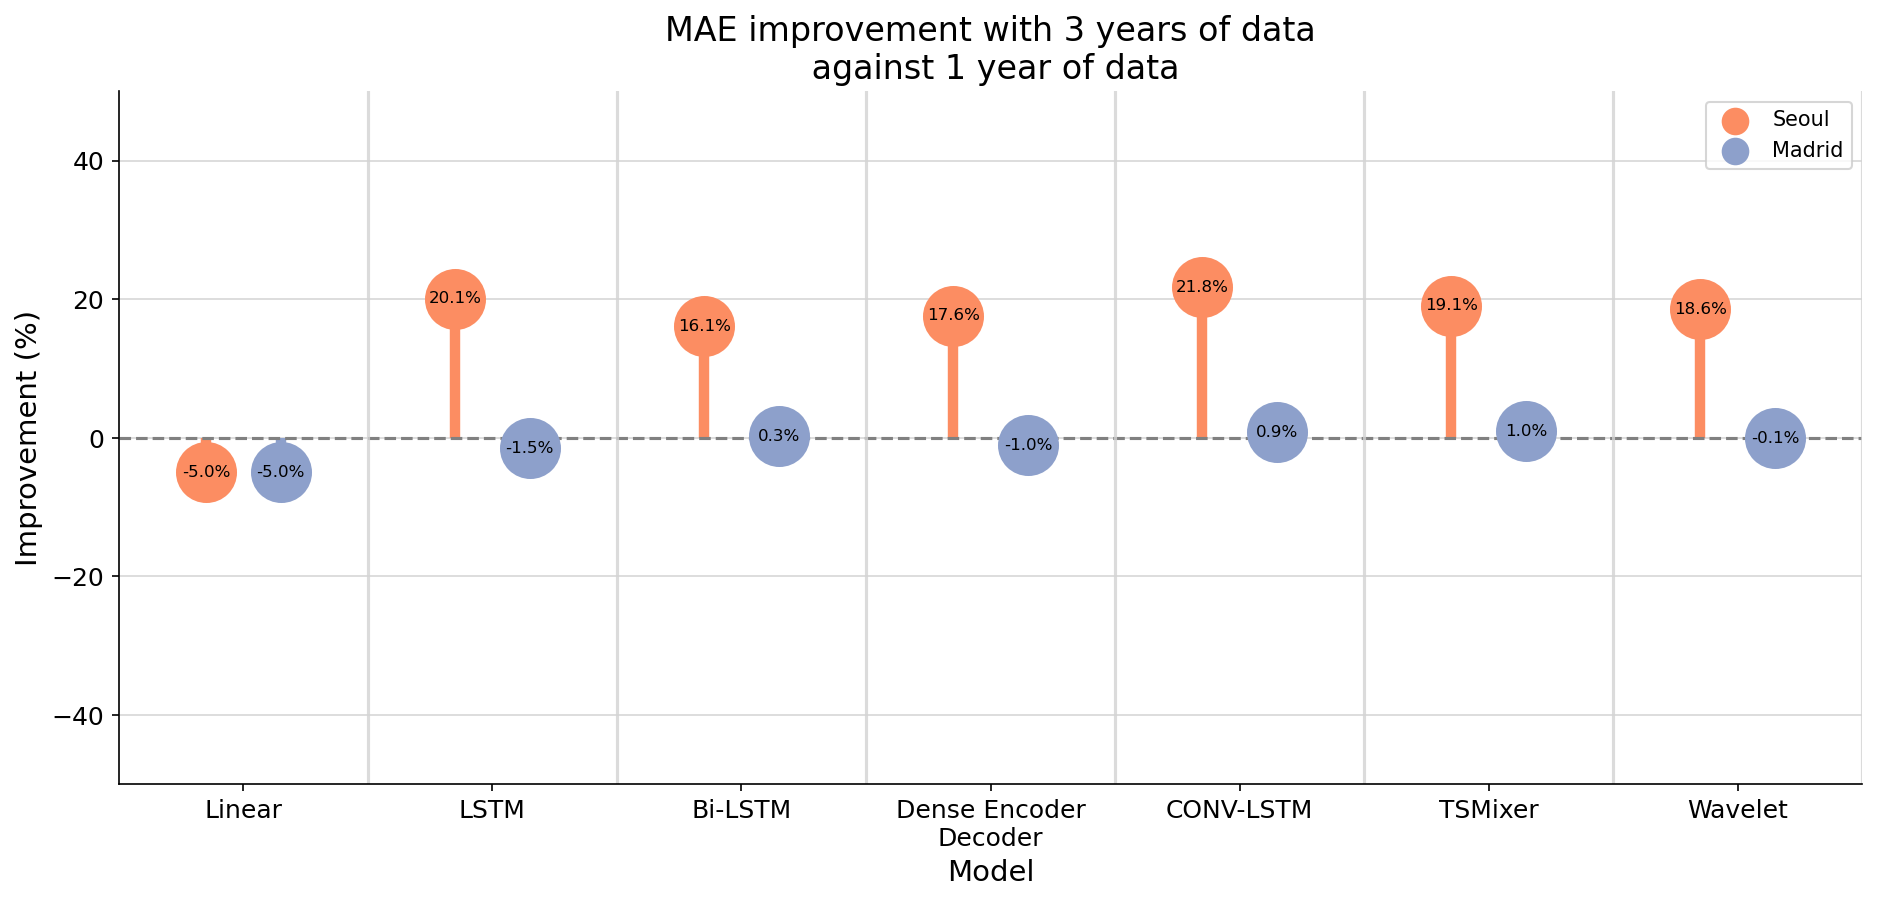
\includegraphics[width=1\linewidth]{images/improvement with more data.png}
    \caption{Reduction in MAE (\%) in models trained with 3 years of data, compared with that with 1 year of data.}
    \label{fig:more_data_improv}
\end{figure}

A clear improvement of approximately 20\% is evident across all models, except for the Linear model. This observation supports the claim that the simplicity of the Linear model hinders its adaptability to a non-uniform dataset. It is noteworthy that the other models benefit significantly from an expanded training dataset, with the CONV-LSTM model showing the most substantial improvement at 21.8\%. This result supports the idea that as the model becomes more complex, more training data is needed to achieve the best performance.

\paragraph{Data augmentation benefits}

In this chapter we have seen that data augmentation have brought benefits in the predictions. The following plot (Figure \ref{fig:augmentation-improv}) is used to better understand the impact of the implemented data augmentation on the results, for each model, in the three datasets.

\begin{figure}[h]
    \centering
    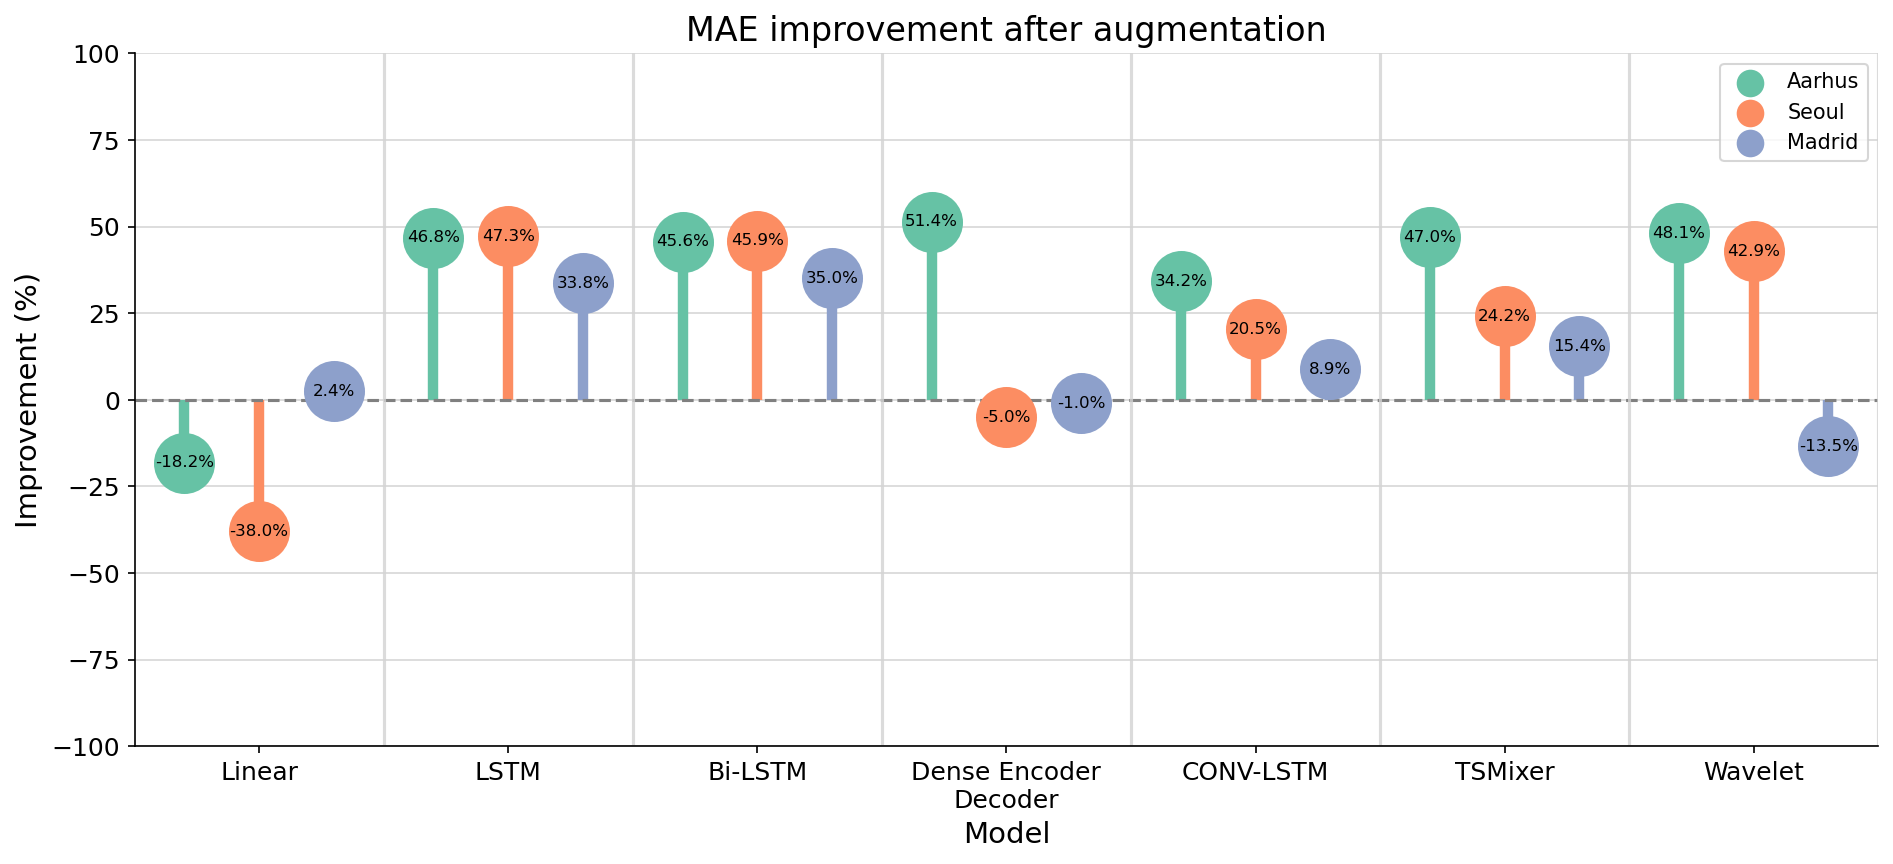
\includegraphics[width=1\linewidth]{images/improvement with augmentation.png}
    \caption{MAE reduction (\%) after data augmentation, for all models.}
    \label{fig:augmentation-improv}
\end{figure}

Despite the worstening in the linear model, for which we have already given an explanation in the previous sections, what we see is that overall the data augmentation confirms it's utility in the training process, with also reductions of almost -50\% in MAE. 






% VA NELLE CONCLUSIONI




